% Author: Max Melching, 2025
% Lots of styling inspiration from: https://tikz.net/relativity_minkowski_diagram/
\documentclass[border=3pt,tikz]{standalone}

\usepackage{newtxmath}  % Use Times in math mode
\usepackage{tgpagella}  % Use Pagella in text
\usepackage{tikz}
\usepackage{fp}
\usepackage{calc}
\usepackage{pgfkeys}
\usepackage{ifthen}
\usepackage{xcolor}
\usepackage[outline]{contour} % glow around text


\usetikzlibrary{math,arrows.meta,calc,intersections,through,backgrounds,decorations.pathreplacing,decorations.markings,decorations.pathmorphing}


% -- Styling
\colorlet{lightyellow}{black!10!yellow}
\colorlet{mydarkred}{red!55!black}
\colorlet{myred}{red!85!black}
\colorlet{mydarkorange}{orange!85!black}
\colorlet{mydarkblue}{blue!50!black}


\tikzset{
    >={Stealth[inset=0,angle'=27]},
    light/.style={
        ->,
        lightyellow,
        % line width=0.6,
        semithick,
        decorate,
        decoration={
            snake,
            amplitude=0.5,
            segment length=4.2,
            post length=4.2,
        },
    },
    worldline/.style={
        ->,
        thick,
        black,
    },
    labelledpoint/.style={
        % mydarkred,
        myred,
    },
    simultline/.style={
        mydarkblue,
        dashed,
        % line width=0.4,
        thin,
    },
    ruler/.style={
        thick,
        % mydarkblue,
        mydarkorange,
    },
}


% -- Not styling, this is to Lorentz-transform objects
\tikzset{
    vlorentz/.style={
      cm={1/((1-((#1)*(#1)))^.5,#1*1/((1-((#1)*(#1)))^.5,#1*1/((1-((#1)*(#1)))^.5,1/((1-((#1)*(#1)))^.5,(0,0)}
    },
}



\begin{document}

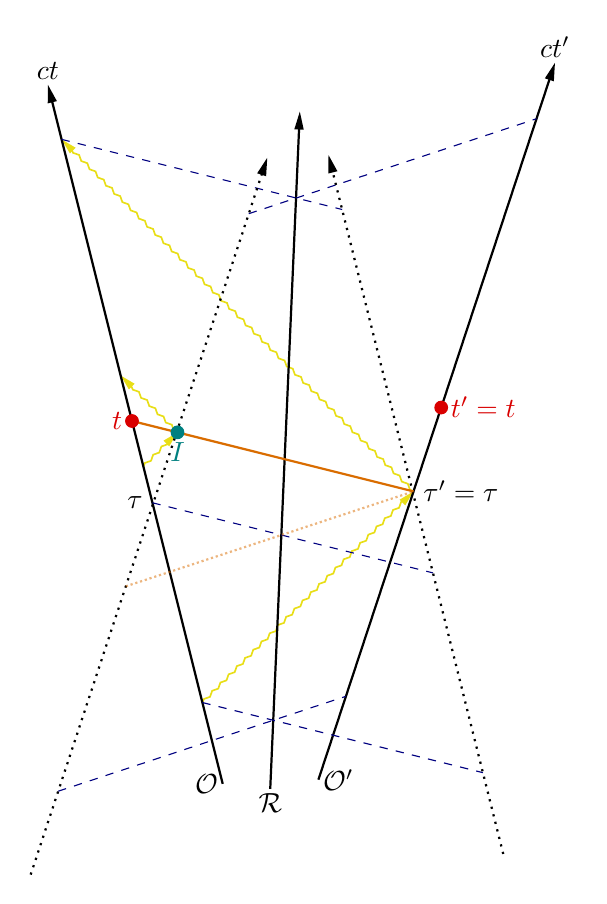
\begin{tikzpicture}

    % -- Set these values to your liking
    \def\vone{0.0}
    \def\vtwo{0.4}
    \def\rulerlength{2}  % So that left end of O rod and left end of O' rod tough in \tau -> TODO: there must be a way to calculate this
    
    \def\tsignalone{3}
    \def\tsignaltwo{\tsignalone}
    % -- tsignaltwo must be equal to tsignalone for synchrony; change if you want to show how desynchronized observers look like
    % \def\tsignaltwo{2.5}
    \def\initsep{0}


    \def\tmin{2}
    \def\tmax{7.6}




    
    \def\vone{-0.15}
    \def\vtwo{0.25}
    \def\rulerlength{1.87}  % So that left end of O rod and left end of O' rod tough in \tau -> TODO: there must be a way to calculate this
    
    \def\tsignalone{3}
    \def\tsignaltwo{\tsignalone}
    % -- tsignaltwo must be equal to tsignalone for synchrony; change if you want to show how desynchronized observers look like
    % \def\tsignaltwo{2.5}
    \def\initsep{0}


    \def\tmin{2}
    \def\tmax{7.6}





    %  -- Trying to mimick Dragon Fig. 2.11
    \def\vone{-0.25}
    \def\vtwo{0.33}
    \def\rulerlength{3.45}  % So that left end of O rod and left end of O' rod tough in \tau -> TODO: there must be a way to calculate this
    
    \def\tsignalone{3}
    \def\tsignaltwo{\tsignalone}
    % -- tsignaltwo must be equal to tsignalone for synchrony; change if you want to show how desynchronized observers look like
    % \def\tsignaltwo{2.5}
    \def\initsep{0}


    \def\tmin{2}
    \def\tmax{10.6}





    % \clip (0, 2.8) rectangle (4, 8);  % If you don't like how long certain lines extend

    
    % -- From here on automatic (except you wish to change styling) -----------
    \FPeval{\dopplerone}{((1+\vone)/(1-\vone))^.5}
    \FPeval{\dopplertwo}{((1+\vtwo)/(1-\vtwo))^.5}
    \FPeval{\doppleronetwo}{\dopplertwo/\dopplerone}

    
    \FPeval{\vrelative}{(\vtwo-\vone)/(1-\vone*\vtwo)}
    
    \FPifzero{\vrelative}
        % -- Only initsep is present, just set sensible values
        \FPeval{\vrelativehalf}{0}
        \FPeval{\vreferee}{\vone}
    \else
        \FPeval{\vrelativehalf}{(1-(1-\vrelative*\vrelative)^.5)/\vrelative}
        \FPeval{\vreferee}{(\vone+\vrelativehalf)/(1+\vone*\vrelativehalf)}
    \fi


    \FPeval{\tauval}{\doppleronetwo*\tsignalone}
    \FPeval{\tval}{(\doppleronetwo*\doppleronetwo*\tsignalone+\tsignalone)/2}
    

    % -- Calculate relevant coordinates
    \begin{scope}[vlorentz=\vone]
        \coordinate (Al) at (0, \tsignalone);
        \coordinate (El) at (0, \doppleronetwo*\tsignalone + \initsep);
        \coordinate (Bl) at (0, \doppleronetwo*\doppleronetwo*\tsignalone + 2*\initsep);
        \coordinate (ABhalfl) at ($ (Al)!0.5!(Bl) $);
        
        \coordinate (Ar) at (\rulerlength, \tsignalone);
        \coordinate (Er) at (\rulerlength, \doppleronetwo*\tsignalone + \initsep);
        \coordinate (Br) at (\rulerlength, \doppleronetwo*\doppleronetwo*\tsignalone + 2*\initsep);
        \coordinate (ABhalfr) at ($ (Ar)!0.5!(Br) $);
    \end{scope}

    \begin{scope}[vlorentz=\vtwo]
        \coordinate (Cl) at (\initsep - \rulerlength, \tsignalone);
        \coordinate (Fl) at (\initsep - \rulerlength, \doppleronetwo*\tsignalone + \initsep);
        \coordinate (Dl) at (\initsep - \rulerlength, \doppleronetwo*\doppleronetwo*\tsignalone + 2*\initsep);
        \coordinate (CDhalfl) at ($ (Cl)!0.5!(Dl) $);
        
        \coordinate (Cr) at (\initsep, \tsignalone);
        \coordinate (Fr) at (\initsep, \doppleronetwo*\tsignalone + \initsep);
        \coordinate (Dr) at (\initsep, \doppleronetwo*\doppleronetwo*\tsignalone + 2*\initsep);
        \coordinate (CDhalfr) at ($ (Cr)!0.5!(Dr) $);
    \end{scope}



    \FPeval{\tintersect}{0.485}  % TODO: there must be a way to calculate this...
    \begin{scope}[vlorentz=\vone]
        % \coordinate (Pshift) at (0, \doppleronetwo*\tintersect);
        % \coordinate (Pshift) at (0, \doppleronetwo*\tsignalone - \doppleronetwo*\tintersect);
        \coordinate (Pshift) at (0, \tval - \doppleronetwo*\tintersect);
        % \coordinate (Pshift) at (0, \tval);
        % TODO: \initsep might be missing here
        
        \FPeval{\tintersecthalf}{(\doppleronetwo*\doppleronetwo*\tintersect+\tintersect)/2}
        \coordinate (Pshift) at (0, \tval - \tintersecthalf);
    \end{scope}

    \begin{scope}[
        shift={(Pshift)},
    ]
        \begin{scope}[vlorentz=\vone]
            \coordinate (G) at (0, \tintersect);
            \coordinate (H) at (0, \doppleronetwo*\doppleronetwo*\tintersect + 2*\initsep);
        \end{scope}
        
        \begin{scope}[vlorentz=\vtwo]
            \coordinate (I) at (\initsep, \doppleronetwo*\tintersect + \initsep);
        \end{scope}
    \end{scope}
    
    
    % -- Light signals. Separate paths instead of A-F-B for styling reasons
    \draw[light] (Al) -- (Fr);
    \draw[light] (Fr) -- (Bl);
        
    % \draw[light] (C) -- (E);
    % \draw[light] (E) -- (D);

    \draw[light] (G) -- (I);
    \draw[light] (I) -- (H);
    
    
    % -- Observer worldlines
    \begin{scope}[
        worldline,
    ]
        \draw[vlorentz=\vone] (0, \tmin) node[left=-2] {$\mathcal{O}$} -- (0, \tmax) node[above=-2] {\contour{white}{$ct$}};

        \draw[vlorentz=\vtwo] (\initsep, \tmin) node[right=-2] {$\mathcal{O}'$} -- (\initsep, \tmax) node[above=-2] {\contour{white}{$ct'$}};

        \draw[vlorentz=\vreferee] ({\initsep/2}, \tmin) node[below=-2] {\contour{white}{$\mathcal{R}$}} -- ({\initsep/2}, \tmax);
    \end{scope}
    

    % -- Lines of Simultaneity
    \begin{scope}[
        simultline,
    ]
        % \draw (A) -- (C);
        % \draw (B) -- (D);
        % \draw (E) -- (F);
        % \draw (ABhalf) -- (CDhalf);

        \draw (Al) -- (Ar);
        \draw (Bl) -- (Br);
        \draw (Cl) -- (Cr);
        \draw (Dl) -- (Dr);
        \draw (El) -- (Er);
        % \draw (Fl) -- (Fr);
    \end{scope}

    % -- Mirrors of observers
    \begin{scope}[
        worldline,
        % densely dotted,
        dotted,
        % opacity=0.4,
    ]
        % \draw (Al) -- (Ar);
        
        % \draw[vlorentz=\vone] (\rulerlength, \tmin) node[left=-2] {$\mathcal{O}$} -- (\rulerlength, \tmax) node[above=-2] {\contour{white}{$ct$}};
        \draw[vlorentz=\vone] (\rulerlength, \tmin) -- (\rulerlength, \tmax);

        % \draw[vlorentz=\vtwo] (\initsep - \rulerlength, \tmin) node[right=-2] {$\mathcal{O}'$} -- (\initsep - \rulerlength, \tmax) node[above=-2] {\contour{white}{$ct'$}};
        \draw[vlorentz=\vtwo] (\initsep - \rulerlength, \tmin) -- (\initsep - \rulerlength, \tmax);
    \end{scope}


    % -- Rulers
    \begin{scope}[
        ruler,
    ]
        \draw (ABhalfl) -- (Fr);
        \draw[
            densely dotted,
            % dotted,
            opacity=0.5,
        % ] (CDhalfr) -- (El);
        ] (Fl) -- (Fr);
    \end{scope}


    % -- Point halfway between emission and reception (= \tau = \tau' if no relative velocity between O, O')
	\draw[fill, labelledpoint] (ABhalfl) circle(0.08);
	\draw[fill, labelledpoint] (CDhalfr) circle(0.08);


    % -- Labels. Comment if you do not like
    \node[left, labelledpoint] at (ABhalfl) {\contour{white}{$t$}};
    \node[right, labelledpoint] at (CDhalfr) {\contour{white}{$t' = t$}};

    \node[left] at (El) {\contour{white}{$\tau$}};
    \node[right] at (Fr) {\contour{white}{$\tau' = \tau$}};

    \draw[fill, teal] (I) circle(0.08) node[below] {\contour{white}{$I$}};
\end{tikzpicture}



\end{document}